% Ceci est le dernier fichier TeX pour le cours de mathématiques financière.
% J'ai eu un problème d'encodage sur mon fichier principal, ce qui m'oblige à
% créer un dernier fichier pour le dernier cours qui va être indépendant!
\documentclass[12pt, french]{report}

% !TEX encoding = UTF-8 Unicode
% LaTeX Preamble
% Author : Gabriel Crépeault-Cauchon
% Last update : 08/09/2019
% ---------------------------------------------
% BEGINNING OF PREAMBLE
% ---------------------------------------------
% Encoding packages
\usepackage[utf8]{inputenc}
\usepackage[T1]{fontenc}
\usepackage{babel}
\usepackage{lmodern}

% HYPERREF (URL's and Link options)
\usepackage{hyperref}
\hypersetup{colorlinks = true, urlcolor = red!60!black, linkcolor = red!60!black}

% POLICY (choose one of them)
%	\usepackage{concrete}
%	\usepackage{mathpazo}
%	\usepackage{frcursive} %% permet d'écrire en lettres attachées
 \usepackage{aeguill}
% 	\usepackage{mathptmx}
%	\usepackage{fourier} 

% Mathematics configuration
\usepackage{amsmath,amsthm,amssymb,latexsym,amsfonts}
\usepackage{empheq}
\usepackage{numprint}
\usepackage{dsfont} 


% Tcolorbox config
\usepackage{tcolorbox}
\tcbuselibrary{xparse}
\tcbuselibrary{breakable}

% Définition Boite pour exemple
\newcounter{ex}[section]
\DeclareTColorBox{exemple}{ o }% #1 parameter
{colframe=green!20!black,colback=green!5!white, % color of the box
breakable, pad at break*=0mm, % to split the box
before title = {\textbf{Exemple \stepcounter{ex} \arabic{chapter}.\arabic{section}.\arabic{ex} }},
IfValueTF = {#1}{title= {#1}}{title= \hphantom},
after title = {\large \hfill \faWrench}
}

%% Définition boite pour définition
\newcounter{def}[section]
\DeclareTColorBox{definition}{ o }% #1 parameter
{colframe=blue!60!green,colback=blue!5!white, % color of the box
breakable, pad at break*=0mm, % to split the box
before title = {\textbf{Définition \stepcounter{def} \arabic{chapter}.\arabic{section}.\arabic{def} }},
title = {#1},
after title = {\large \hfill \faBook}
}

\DeclareTColorBox{note}{ o }
    {colframe=black,
     colback=white,
     sharp corners,
     pad at break*=0mm,
     IfValueTF={#1}{title={#1}, fonttitle=\bfseries}{title=Note, fonttitle=\bfseries}}


% Graphics and picture import Packages
\usepackage{graphicx}
\usepackage{pict2e}

% insert PDF package
\usepackage{pdfpages}

% Color package
\usepackage{color, soulutf8, colortbl}

% Mathematics table
\usepackage{array}   % for \newcolumntype macro
\newcolumntype{L}{>{$}l<{$}} % math-mode version of "l" column type

% usefull shortcut for colored text
\newcommand{\orange}{\textcolor{orange}}
\newcommand{\red}{\textcolor{red}}
\newcommand{\cyan}{\textcolor{cyan}}
\newcommand{\blue}{\textcolor{blue}}
\newcommand{\green}{\textcolor{green}}
\newcommand{\darkgreen}{\textcolor{darkgreen}}
\newcommand{\purple}{\textcolor{magenta}}
\newcommand{\yellow}{\textcolor{yellow}}

% Colors define
\definecolor{darkgreen}{RGB}{37, 128, 40}
\definecolor{tocColor}{HTML}{8A2507}

% Custum enumerate & itemize Package
\usepackage{enumitem}
% French Setup for itemize function
\frenchbsetup{StandardItemLabels=true}

% Mathematics shortcut
\usepackage{cancel}
\newcommand{\reels}{\mathbb{R}}
\newcommand{\entiers}{\mathbb{Z}}
\newcommand{\naturels}{\mathbb{N}}
\newcommand{\eval}{\biggr \rvert}
\newcommand{\esp}[1]{\mathrm{E} \left[ #1 \right]} % espérance
\newcommand{\variance}[1]{\mathrm{Var} \left( #1 \right)} % variance
\newcommand{\covar}[1]{\mathrm{Cov} \left( #1 \right)} % variance
\newcommand{\prob}[1]{\Pr \left( #1 \right)} % probabilité entre parenthèses
\newcommand{\laplace}{\mathcal{L}}
\newcommand{\matr}[1]{\mathbf{#1}} % Notation matricielle
\DeclareMathOperator{\Tr}{Tr}
\newcommand{\fgp}{\mathcal{P}}
\DeclareMathOperator{\Adj}{Adj}
\newcommand{\derivee}[1]{\frac{\partial}{\partial #1}}
\newcommand{\indic}[1]{\mathds{1}_{\{ #1 \}}}
\newcommand{\VaR}[2][k]{\mathrm{VaR}_{#1}{\left( #2 \right)}}
\newcommand{\TVaR}[2][k]{\mathrm{TVaR}_{#1}{\left( #2 \right)}}


% Matricial anotation for math symbols (\bm{•})
% à enlever éventuellement, j'ai ajouté la macro \matr{} à la place.
\usepackage{bm}

% Actuarial notation package
\usepackage{actuarialsymbol}
\usepackage{actuarialangle}

% To indicate equation number on a specific line in align environment
\newcommand\numberthis{\addtocounter{equation}{1}\tag{\theequation}}

% Other shortcut
\newcommand{\p}{\paragraph{}}
\newcommand{\n}{\newline}

% source : https://tex.stackexchange.com/questions/112576/math-mode-in-tabular-without-having-to-use-everywhere



% Special symbols package
 \usepackage[tikz]{bclogo}
\usepackage{fontawesome}

% Retire l'indentation automatique de Latex
\setlength{\parindent}{0pt}

% Utilisé pour la page couverture
\usepackage[absolute]{textpos} % Textblock environement
\usepackage{anyfontsize} % Avoir un gros titre
\usepackage{titling} % Avoir un gros titre
\usepackage{changepage} % ajustwidth environement

% Pour afficher du code
\usepackage{listings}

\definecolor{codegray}{gray}{0.9}
\newcommand{\code}[1]{\colorbox{codegray}{\texttt{#1}}}

\definecolor{insideBlackTerminal}{RGB}{33,33,33}
% Set Language
% \lstset{
%     language={bash},
%     basicstyle=\small\ttfamily\color{white}, % Global Code Style
%     captionpos=b, % Position of the Caption (t for top, b for bottom)
%     extendedchars=true, % Allows 256 instead of 128 ASCII characters
%     tabsize=2, % number of spaces indented when discovering a tab 
%     columns=fixed, % make all characters equal width
%     keepspaces=true, % does not ignore spaces to fit width, convert tabs to spaces
%     showstringspaces=false, % lets spaces in strings appear as real spaces
%     breaklines=true, % wrap lines if they don't fit
%     frame=single, % draw a frame at the top, right, left and bottom of the listing
%     numberstyle=\tiny\ttfamily, % style of the line numbers
%     % commentstyle=\color{red}, % style of comments
%     % keywordstyle=\color{red}, % style of keywords
%     % stringstyle=\color{red}, % style of strings
%     backgroundcolor = \color{insideBlackTerminal},
%     rulecolor=\color{red}
% }

\usepackage{lstlinebgrd}
\definecolor{grayComment}{HTML}{8D90B8}
\lstset{
language=R,                     % the language of the code
basicstyle=\ttfamily, % the size of the fonts that are used for the code
% numbers=left,                   % where to put the line-numbers
% numberstyle=\color{blue},  % the style that is used for the line-numbers
% stepnumber=1,                   % the step between two line-numbers. If it is 1, each line
% will be numbered
numbersep=5pt,                  % how far the line-numbers are from the code
backgroundcolor=\color{white},  % choose the background color. You must add \usepackage{color}
linebackgroundcolor=\color{white},
showspaces=false,               % show spaces adding particular underscores
showstringspaces=false,         % underline spaces within strings
showtabs=false,                 % show tabs within strings adding particular underscores
frame=single,                   % adds a frame around the code
rulecolor=\color{black},        % if not set, the frame-color may be changed on line-breaks within not-black text (e.g. commens (green here))
tabsize=2,                      % sets default tabsize to 2 spaces
captionpos=b,                   % sets the caption-position to bottom
breaklines=true,                % sets automatic line breaking
breakatwhitespace=false,        % sets if automatic breaks should only happen at whitespace
%   keywordstyle=\color{functionR},      % keyword style
commentstyle=\color[HTML]{9F0808},  %\color[HTML]{8D90B8},   % comment style
%   stringstyle=\color[HTML]{1D9507},      % string literal style
moredelim=**[is][\color{grayComment}]{@}{@}, % couleur manuel
literate=%
{à}{{\`a}}1
{é}{{\'e}}1
{è}{{\`e}}1
} 




















































% ---------------------------------------------
% END OF PREAMBLE
% ---------------------------------------------



% Pr�sentation document
	\title{Notes du dernier cours \\ Mathématiques financières \\ Automne 2017 \\ ACT-1001}
	\author{Gabriel Crépeault-Cauchon}
	\date{Dernière mise à jour : \today}

% Mise en page du document
\usepackage{fancyhdr}
\pagestyle{fancy}
\fancyhead{}
\fancyhead[L]{\text{Dernier cours ACT-1001}}
\fancyhead[R]{\today}
\fancyfoot{}
\fancyfoot[RO,RE]{\thepage}
\renewcommand{\footrulewidth}{0.5pt}


% Commencer la numérotation des chapitres
\setcounter{chapter}{6}
% fin du pr�ambule


% ------------------------------------------------------------------------------
\begin{document}

% ------------------------------------------------------------------------------
\part*{Notes du dernier cours ACT-1001}


\chapter{Duration et immunisation}
\setcounter{section}{1}		% pour considérer les chapitres passés

\section{Appariement et immunisation}
Anglais :
\begin{itemize}
	\item Immunisation : \emph{Immunization}
	\item Appariement  : \emph{Asset-Liability matching (ALM)}
\end{itemize}
\p
Notation à utiliser :
\begin{itemize}
	\item $L_t$ : flux de passif (\emph{liabilities})
	\item $A_t$ : flux d'actif (\emph{assets})
\end{itemize}

\bcsmbh On suppose une structure plate ($s_0(t) = i \forall\ t$) et qu'on est
dans un marché efficient (on emprunte et investit au même taux).
\p
Objectif : on veut minimiser l'impact d'un changement dans le taux d'intérêt sur
la situation de la compagnie. On peut le faire par appariement, soit
\begin{displaymath}
	A_t = L_t \quad \forall\ t
\end{displaymath}
Dans le même sens,
\begin{displaymath}
	\sum_{t=0}^n (A_t - L_t)(1+i)^{-t} = 0
\end{displaymath}
Ce qui signifie qu'en changeant le taux d'intérêt, les $VA_A$ et $VA_L$ vont
changer, mais leur différence va toujours être égale à zéro. Nous en rediscuterons
dans la section sur l'immunisation complète (\ref{subsec:immunisation_complete}).
\p
Sans surprise,
\begin{equation}
	VA_A = \sum_{t=0}^n A_t(1+i)^{-t}
\end{equation}
\begin{equation}
	VA_L = \sum_{t=0}^n L_t(1+i)^{-t}
\end{equation}

\subsubsection*{Exemple}
On connaît $L_1 =1, \quad L_2 = 2, \quad L_3 = 3$. On veut savoir combien
d'obligations à coupon \emph{annuel} de 2\% il nous faut, selon leur échéance.
Les obligations sont notées $A_1, A_2$ et $A_3$, où $A_n$ est une obligation avec
échéance dans $n$ années. Pour les fins de l'exemple, on suppose un marché efficient
où l'on peut acheter des fractions d'obligations.
\p
On représente $\alpha_n$ comme le nombre d'obligation qui a échéance dans $n$ années.
\begin{align*}
	A_1	& = 2 \alpha_3		& + 2 \alpha_2			& + 102 \alpha_1			& = 1 \\
	A_2	& = 2 \alpha_3		& + 102 \alpha_2		& 										& = 1 \\
	A_3	& = 102 \alpha_3	& 									& 										& = 1 \\
\end{align*}
C'est un système d'équation très simple à résoudre en commencant par le flux d'actif $A_3$.


\subsection{Immunisation selon Redington}
\bcsmbh Encore une fois, cette section est dans un contexte de Structure plate.

\bcattention L'immunisation selon reddington fonctionne dans le cas où les taux
subissent un choc instantanée, mais que la structure reste néanmoins plate.
\begin{center}
	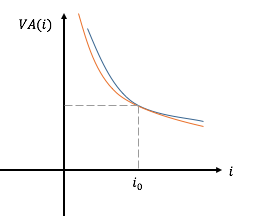
\includegraphics[width = 5cm, height = 5cm]{Reddington_graph.png}
\end{center}
Pour dire qu'on est immunisé, on désire que $VA_A > VA_L$ au taux actuel $i_0$ donné.
Toutefois, si on veut une immunisation totale en tout point, le flux d'actif doit
être plus convexe que le flux de passif. Bref, voici les 3 conditions de Redington
à respecter :

\begin{align}
	VA_A(i_0) 										& = VA_L(i_0) \\
	\frac{d}{di} VA_A	\eval_{i=i_0}			& = \frac{d}{di} VA_L \eval_{i = i_0} \\
	\frac{d^2}{di^2} VA_A \eval_{i=i_0}		& = \frac{d^2}{di^2} VA_L \eval_{i=i_0} \\
\end{align}
On peut ré-écrire ces 3 conditions de 2 autres façons :
\begin{align}
	VA_A(i_0) 				& = VA_L \\
	D_A(i_0)					& = D_L(i_0) \\
	C_A(i_0)					& = C_A(i_0) \\
\end{align}
\begin{align}
	VA_A(i_0) 				& = VA_L \\
	MD_A(i_0)					& = MD_L(i_0) \\
	MC_A(i_0)					& = MC_A(i_0) \\
\end{align}
\bcattention L'immunisation de Reddington ne fonctionne que pour un \underline{petit} choc.
\p
On pose donc les 2 premières conditions, puis on isole $A_{t_2}$ et $A_{t_2}$ Dans
les équations. Finalement, on valide la 3\up{e} condition pour la dérivée seconde.

\subsection{Immunisation complète}
\label{subsec:immunisation_complete}
en anglais : \emph{Full Immunization}.
\p
Définition : Les flux d'actifs immunisent complètement les flux de passif si
\begin{equation}
	VA_A(i) \ge VA_L(i) \quad \forall\ i >0
\end{equation}
\p
Remarque : l'immunisation, qu'elle soit complète ou selon Redington, requiert en
pratique des ajustements périodiques.
\p
La preuve mathématique a été faite en cours (je l'épargne ici) que si on a des
flux de passifs $L_t \quad t = r,r+1,...s-1,s$, ces derniers seront complètement
immunisés par des flux d'actifs $A_{t_1} \quad t_1 \le r$ et $A_{t_2} \quad t_2 \ge s$
si les 2 premières conditions de Redington sont respectées, soit
\begin{gather*}
	VA_A(i_0) = VA_L(i_0) \\
	t_1 A_{t_1}(1+i_0)^{-t_1} + t_2 A_{t_2} (1+i_0)^{-t_2} = \sum_{t=r}^s t L_t (1+i_0)^{-t} \\
\end{gather*}


% Fin du chapitre 7
\setcounter{chapter}{8}
\chapter{Sujets avancés en finance}
Dans le cadre du cours ACT-1001, on en voit qu'un seul : le modèle d'évaluation
des actions par l'actualisation des dividendes
\blue{(\href{https://www.investopedia.com/terms/d/ddm.asp}{Dividend Discount Model})}.

\section{Modèle d'évaluation des actions par l'actualisation des dividendes}
Tout d'abord, un peu de vocabulaire :
\begin{description}
	\item[Bid] cours acheteur (Prix offert le plus élevé) ;
	\item[Ask] cours vendeur (Prix demandé le plus faible) ;
	\item[Spread] écart acheteur-vendeur (différence entre le \emph{Bid} et le \emph{Ask}).
\end{description}
On a déjà vu les formules suivantes lorsqu'on a parlé de somme géométrique dans
le chapitre 2. $P$ est le prix de l'action, $d_t$ représente la dividende versé
au moment $t$ et $g$ représente le taux de croissance du dividende (s'il y a lieu).
\p
\subsection*{En présence d'une structure plate}

Si on a une structure plate ($i_t = i \forall\ t$) :
\begin{equation}
	P = \frac{d_1}{i - g}
\end{equation}

\subsection*{En présence d'une autre structure des taux}
Si on connaît nos taux au comptant (\emph{spot}):
\begin{equation}
	P = \sum_{t=1}^\infty d_t [1 + s_0(t)]^{-t}
\end{equation}

Si on connaît nos taux à terme (\emph{forward}) :
\begin{equation}
	P = \sum_{t=1}^\infty \prod_{u=1}^\infty \frac{d_t}{1 + i_0(u-1,u)}
\end{equation}







% ------------------------------------------------------------------------------
% Fin du document
\end{document}
% ------------------------------------------------------------------------------
